\documentclass[10pt]{article}
\usepackage[a4paper,landscape,margin=0.72in]{geometry}
\usepackage[T1]{fontenc}
\usepackage{lmodern,amsmath,amssymb,graphicx,hyperref}
\title{Whole weighted-Proj integrality under a separable quintic}
\author{Formal proof packet}
\date{28 October 2026}
\begin{document}
\maketitle
\noindent Pinned Lean 4.34.1 checks that the actual weighted-$\operatorname{Proj}$ curve is integral for any field and coefficient tuple when its quintic is separable. The direct axiom audit of the three new theorems lists only \texttt{propext}, \texttt{Classical.choice}, and \texttt{Quot.sound}. The theorem has no additional characteristic restriction.

\section*{Checked proof structure}
The infinity-chart ring is a domain for every field, and the affine-chart ring is a domain under separability. Two new theorems transport these facts through the checked scheme isomorphisms to the actual $X$- and $Z$-basic opens. The previously checked overlap point and two-open cover supply a pairwise nonempty open cover. The whole-curve theorem applies pinned Mathlib's gluing of preirreducibility and reducedness, then its equivalence of integral schemes with reduced irreducible schemes.

\section*{Scope boundary}
This establishes the scheme-level integrality prerequisite for the function-field API. The source-style common 2+2 function has not been constructed in that field. Its orders over all closed points, principal divisor, Picard-class equality, and compiled Rust correspondence remain open. The accompanying CSV gives each exact status; the Lean source and compiler log give the theorem statements and axiom output. No DLP experiment or cost comparison was run.

\clearpage
\section*{Proof dependencies}
\begin{center}
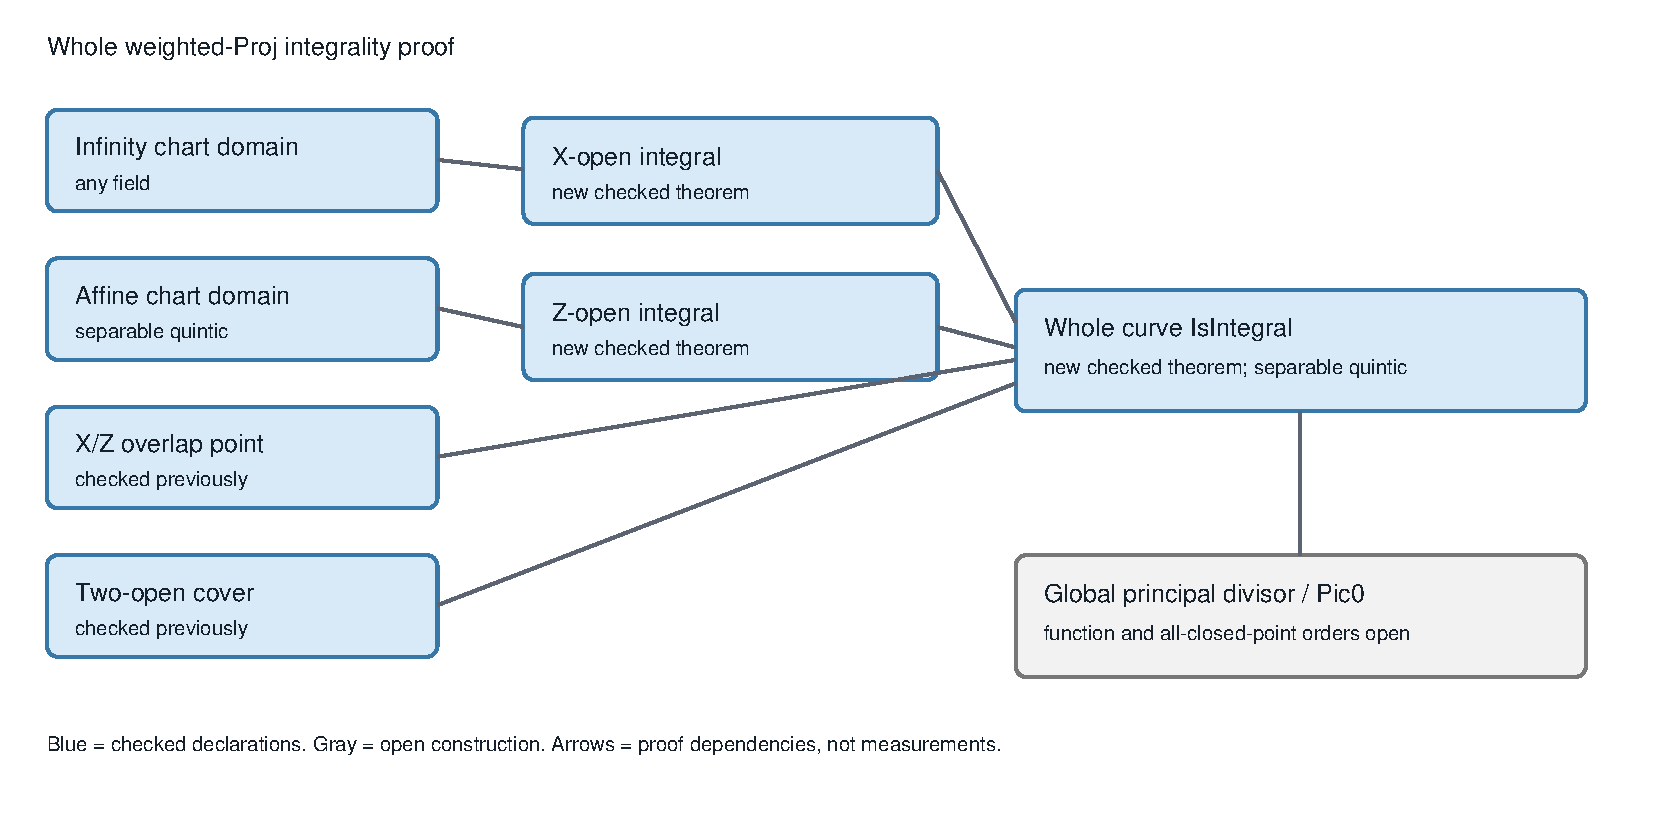
\includegraphics[width=0.96\textwidth,height=0.78\textheight,keepaspectratio]{projective-is-integral-figure.pdf}
\end{center}
\noindent Blue nodes are checked declarations; gray is open construction. Arrows represent proof dependencies, not performance measurements.
\end{document}
